%%%%%%%%%%%%%%%%%%%%%%%%%%%%%%%%%%%%%%%%%%%%%%%%%%%%%%%%%%%%%%%%%%%%%%
% LaTeX Template: Beamer arrows
%
% Source: http://www.texample.net/
% Feel free to distribute this template, but please keep the
% referal to TeXample.net.
% Date: Nov 2006
% 
%%%%%%%%%%%%%%%%%%%%%%%%%%%%%%%%%%%%%%%%%%%%%%%%%%%%%%%%%%%%%%%%%%%%%%
% How to use writeLaTeX: 
%
% You edit the source code here on the left, and the preview on the
% right shows you the result within a few seconds.
%
% Bookmark this page and share the URL with your co-authors. They can
% edit at the same time!
%
% You can upload figures, bibliographies, custom classes and
% styles using the files menu.
%
% If you're new to LaTeX, the wikibook is a great place to start:
% http://en.wikibooks.org/wiki/LaTeX
%
%%%%%%%%%%%%%%%%%%%%%%%%%%%%%%%%%%%%%%%%%%%%%%%%%%%%%%%%%%%%%%%%%%%%%%

\documentclass{beamer}

\usetheme{CambridgeUS}
\usefonttheme{professionalfonts}
\usepackage{times}
\usepackage{tikz}
\usepackage{amsmath}
\usepackage{verbatim}
\usepackage{natbib}
\usepackage[francais]{babel}
\usepackage[T1]{fontenc}
\usepackage[utf8x]{inputenc}
\usepackage{booktabs} % Allows the use of \toprule, \midrule and \bottomrule in tables
\usepackage{graphicx}
\usepackage{wrapfig}
\usepackage{multicol}

\usetikzlibrary{arrows,shapes}
\newcommand{\refimg}[1]{\footnotesize\textit{#1}}

\author{Alexandre Hulsken (CRIStAL / FOX)}
\title{Reconnaissance d'émotions par réseaux de neurones à spikes}


\begin{comment}
:Title: Beamer arrows
:Tags: Remember picture, Beamer, Physics & chemistry, Overlays
:Use page: 3

With PGF/TikZ version 1.09 and later, it is possible to draw paths between nodes across
different pictures. This is a useful feature for presentations with the
Beamer package. In this example I've combined the new PGF/TikZ's overlay feature
with Beamer overlays. Download the PDF version to see the result.

**Note.** This only works with PDFTeX, and you have to run PDFTeX twice.

| Author: Kjell Magne Fauske

\end{comment}


% For every picture that defines or uses external nodes, you'll have to
% apply the 'remember picture' style. To avoid some typing, we'll apply
% the style to all pictures.
\tikzstyle{every picture}+=[remember picture]

% By default all math in TikZ nodes are set in inline mode. Change this to
% displaystyle so that we don't get small fractions.
\everymath{\displaystyle}

\title[Label Recherche]{Reconnaissance d’émotions par réseaux de neurones à Spikes}

\author{Alexandre Hulsken}
\institute[IRCICA/FOX]
{
Université des Sciences et Technologies de Lille \\
\medskip
%\textit{john@smith.com} % Your email address
}
\date{23 mars 2018}

\begin{document}

\begin{frame}
\titlepage
\begin{wrapfigure}{r!}{20mm}

\includegraphics[scale=0.07]{image/logoFOX.png}
\end{wrapfigure}
\vfill
Encadré par :\par
Pierre \textsc{Tirilly} \\
Benjamin \textsc{Allaert}
\end{frame}

%\begin{frame}
%  \frametitle{Sommaire}
%  \tableofcontents
%\end{frame}

%------------------------------------------------
\section{Contexte}
%------------------------------------------------

\subsection{Contexte}
\begin{frame}
  \frametitle{Contexte}
  \begin{picture}(340, 50)
  	\put(0, 0){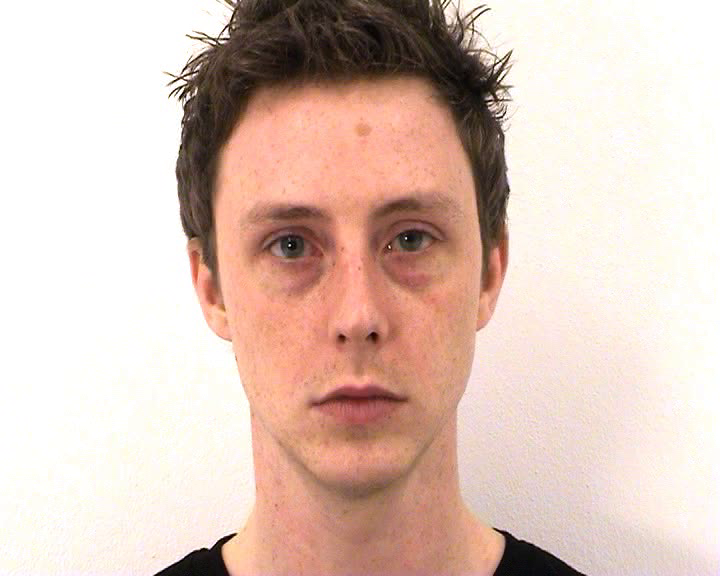
\includegraphics[scale=0.1]{image/img_001.png}}
  	\put(95, 0){\framebox(150, 50){\shortstack{Programme de\\ reconnaissance émotionnelle}}}
    \put(275, 20){\shortstack{ÉMOTION}}
    \put(70, 25){\vector(1, 0){25}}
    \put(245, 25){\vector(1, 0){25}}
  \end{picture}
\end{frame}

%------------------------------------------------

\subsection{Définition}
\begin{frame}
  \frametitle{Définition}
  \begin{block}{Une émotion}
    Classification discrète d'Ekman en 6 classes
  \end{block}
  \begin{figure}
  	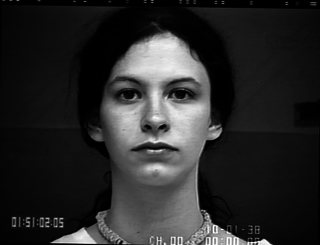
\includegraphics[height=2cm]{image/img_0012_ck.png}
    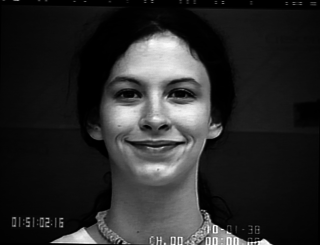
\includegraphics[height=2cm]{image/img_0122_ck.png}
    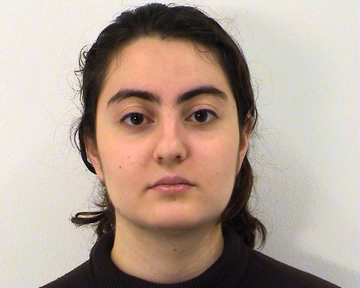
\includegraphics[height=2cm]{image/img_0012_adfes.png}
    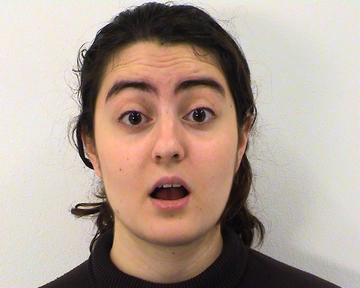
\includegraphics[height=2cm]{image/img_1502_adfes.png}
  \end{figure}
  \refimg{[The extended Cohn-Kanade Dataset (CK+) : A complete dataset for action unit and emotion-specified expression]}\newline
  \refimg{[Moving faces, looking places: Validation of the Amsterdam Dynamic Facial Expression Set (ADFES)]}
\end{frame}

%------------------------------------------------

\subsection{Plusieurs architectures}
\begin{frame}
  \frametitle{Plusieurs architectures}
  Différentes architectures pour cette problématique :
  \begin{enumerate}
    \item Les méthodes dites traditionnelles
    \item Le deep learning
    \item Les réseaux de neurones impulsionnels
  \end{enumerate}
\end{frame}

%------------------------------------------------

\subsection{Problématique}
\begin{frame}
  \frametitle{Problématique}
  \centering
  \huge{Expérimenter les réseaux de neurones à spikes}
\end{frame}

%------------------------------------------------

\subsection{Le principe de reconnaissance d'expressions faciales}
\begin{frame}
  \frametitle{Le principe de la reconnaissance}
  \begin{picture}(340, 200)
  	\put(5, 125){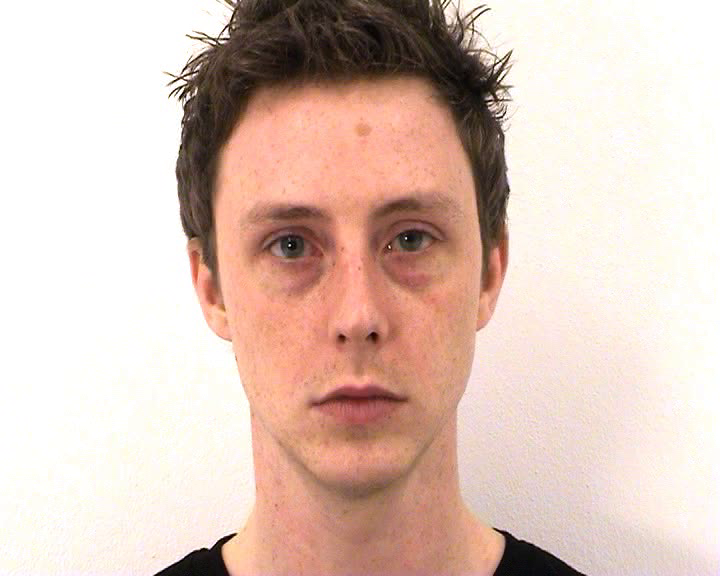
\includegraphics[scale=0.1]{image/img_001.png}}
  	\put(0, 50){\dashbox(340, 50)}
    \put(270, 25){\shortstack{EMOTION}}
    \put(5, 55){\framebox(80, 40){\shortstack{Prétraitement}}}
    \put(130, 55){\framebox(80, 40){\shortstack{Extraction de\\ descripteurs}}}
    \put(255, 55){\framebox(80, 40){Classification}}
    
    \put(40, 125){\vector(0, -1){25}}
    \put(295, 55){\vector(0, -1){18}}
    \put(85, 75){\vector(1, 0){43}}
    \put(210, 75){\vector(1, 0){43}}
  \end{picture}
\end{frame}

%------------------------------------------------ 
\section{Reconnaître une émotion}
%------------------------------------------------

\subsection{Le prétraitement de la donnée}
\begin{frame}
  \frametitle{Le prétraitement}
  \begin{columns}[c] 
    \column{.45\textwidth}
      \textbf{Etapes :}
      \begin{itemize}
        \item Extraction d'une zone
        \item Transformation en niveaux de gris
        \item Extraction de contours
      \end{itemize}

    \column{.5\textwidth}
      \begin{figure}[position]
      	\centering
        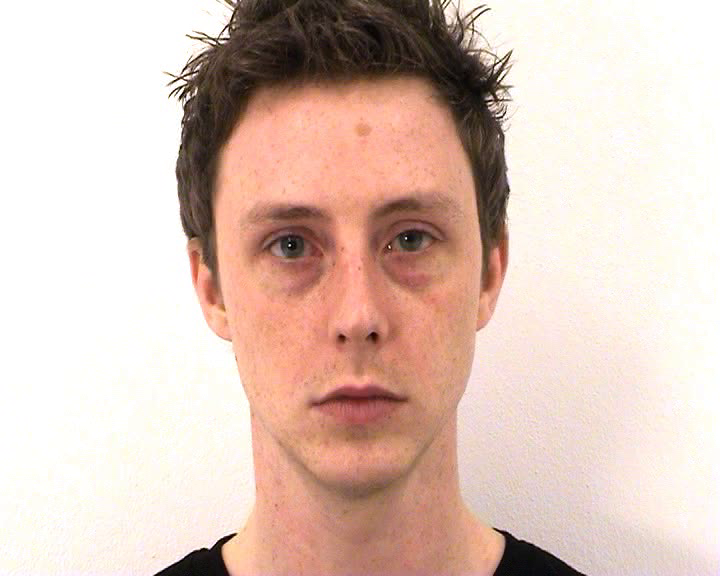
\includegraphics[scale=0.15]{image/img_001.png}
        \vfill
        \vspace{2mm}
        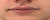
\includegraphics{image/cropped.png}
        \vfill
        \vspace{2mm}
        
\includegraphics{image/grayscale.png}
        \vfill
        \vspace{2mm}
        
\includegraphics{image/dog_on.png}
        \hspace{3mm}
        
\includegraphics{image/dog_off.png}
      \end{figure}
  \end{columns}
\end{frame}

%------------------------------------------------

\subsection{L'extraction de modèles}
\begin{frame}
  \frametitle{Le comportement du neurone}
  \begin{figure}
  	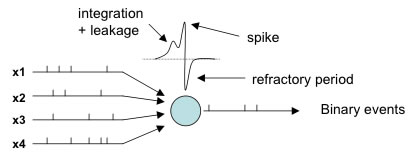
\includegraphics[scale=0.8]{image/neurone.jpg}
  \end{figure}
  \begin{picture}(0, 0)
  	\put(125, 130){\line(1, 0){5}} \put(135, 130){\line(1, 0){5}} \put(145, 130){\line(1, 0){5}} \put(155, 130){\line(1, 0){5}} \put(165, 130){\line(1, 0){5}} \put(175, 130){\line(1, 0){5}}
  \end{picture}
  \refimg{[writelatex.s3.amazonaws.com]}
\end{frame}

%------------------------------------------------

\begin{frame}
  \frametitle{Une architecture de réseau de neurone impulsionnel}
  \begin{figure}
    \centering
    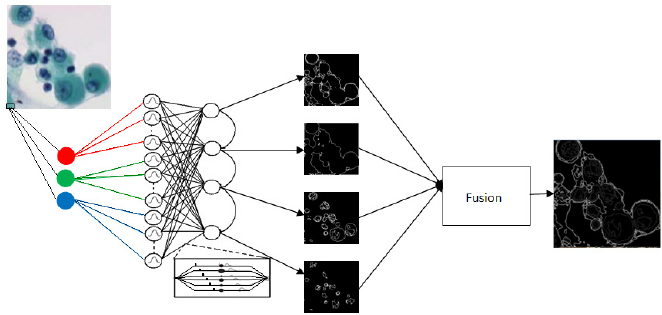
\includegraphics[scale=0.5]{image/SNN1.png}
  \end{figure}
  \refimg{[writelatex.s3.amazonaws.com/]}
\end{frame}

%------------------------------------------------

\subsection{La classification}
\begin{frame}
	\frametitle{La classification}
	\begin{figure}
    	\centering
		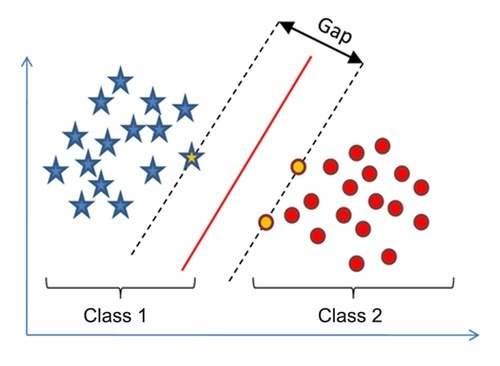
\includegraphics[scale=0.5]{image/svm.jpg}
	\end{figure}
    \refimg{[www.quora.com/How-can-I-use-a-Support-Vector-Machine-in-regression-tasks-SVM}
\end{frame}

%------------------------------------------------
\section{Expérimenter l'architecture}
%------------------------------------------------

\subsection{Test de difficulté}
\begin{frame}
  \frametitle{Test de difficulté}
    \begin{columns}
      \column[c]{.5\textwidth}
        \begin{figure}
        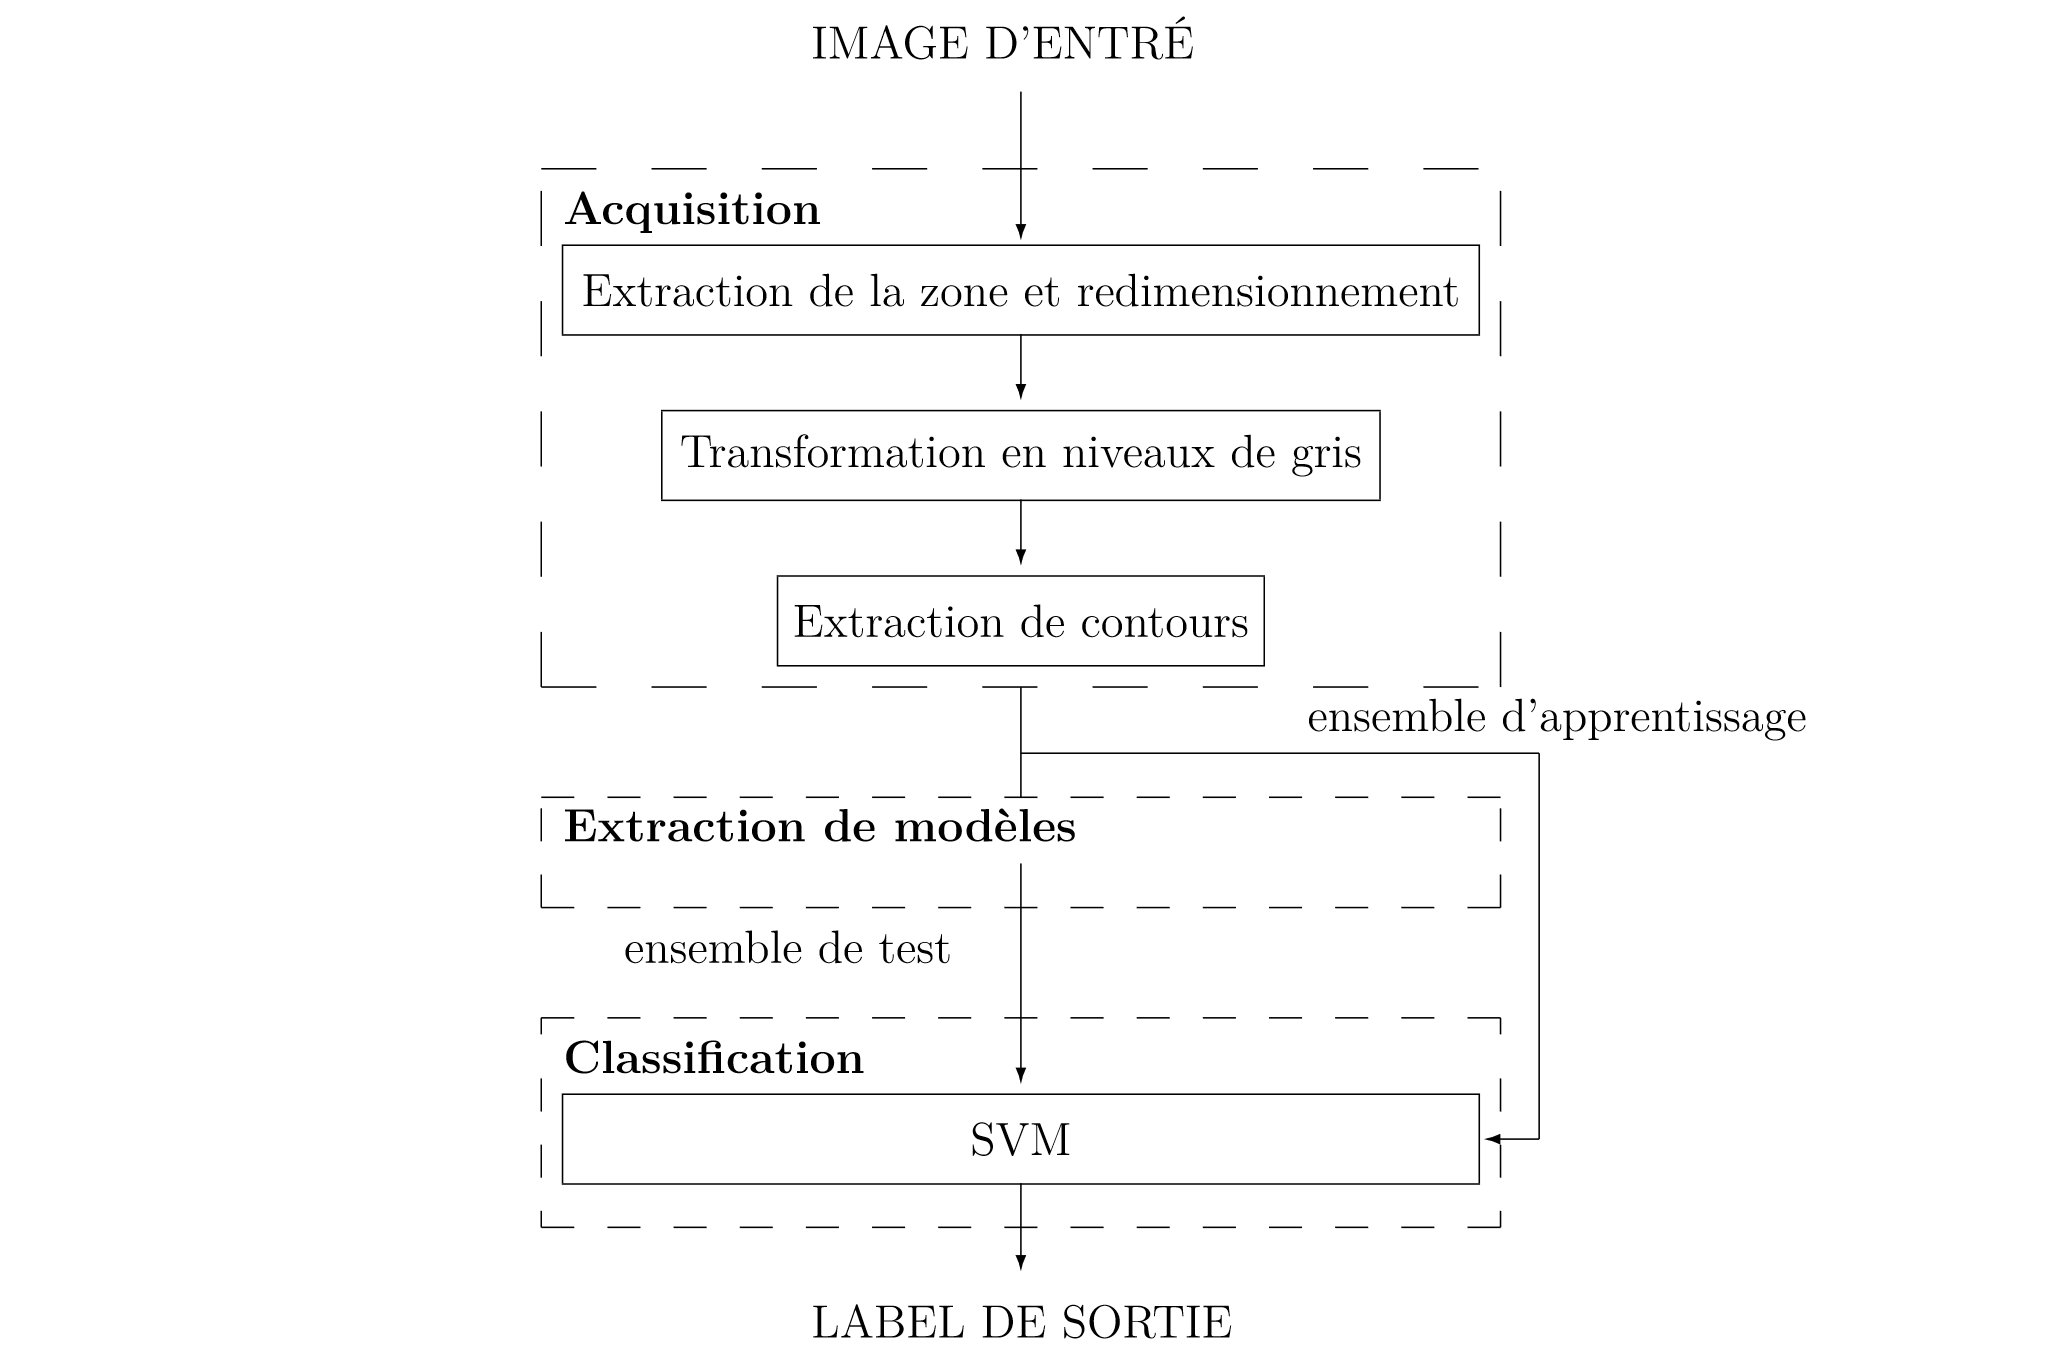
\includegraphics[scale=0.13]{image/test_exp.png}
        \end{figure}

      \column[c]{.55\textwidth}
        \begin{figure}
        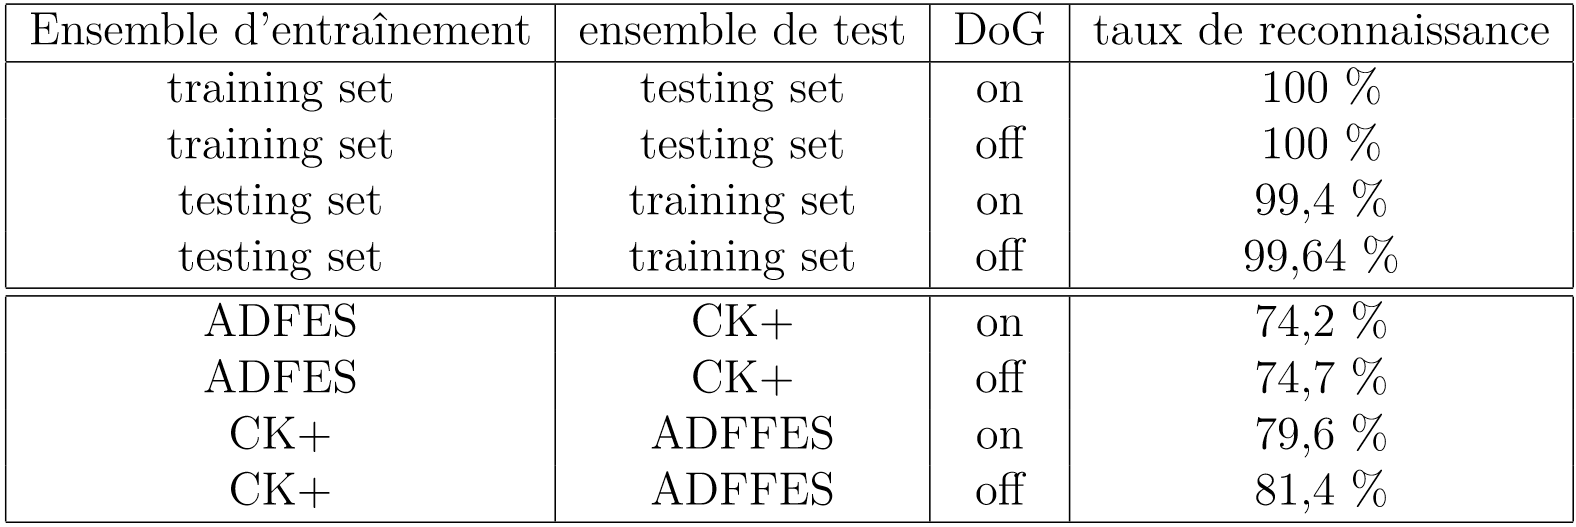
\includegraphics[scale=0.15]{image/resultat_exp.png}
        \end{figure}
    \end{columns}
\end{frame}

%------------------------------------------------

\subsection{Le protocole expérimental}
\begin{frame}
  \frametitle{Le protocole expérimental}
  \begin{figure}
    \centering
    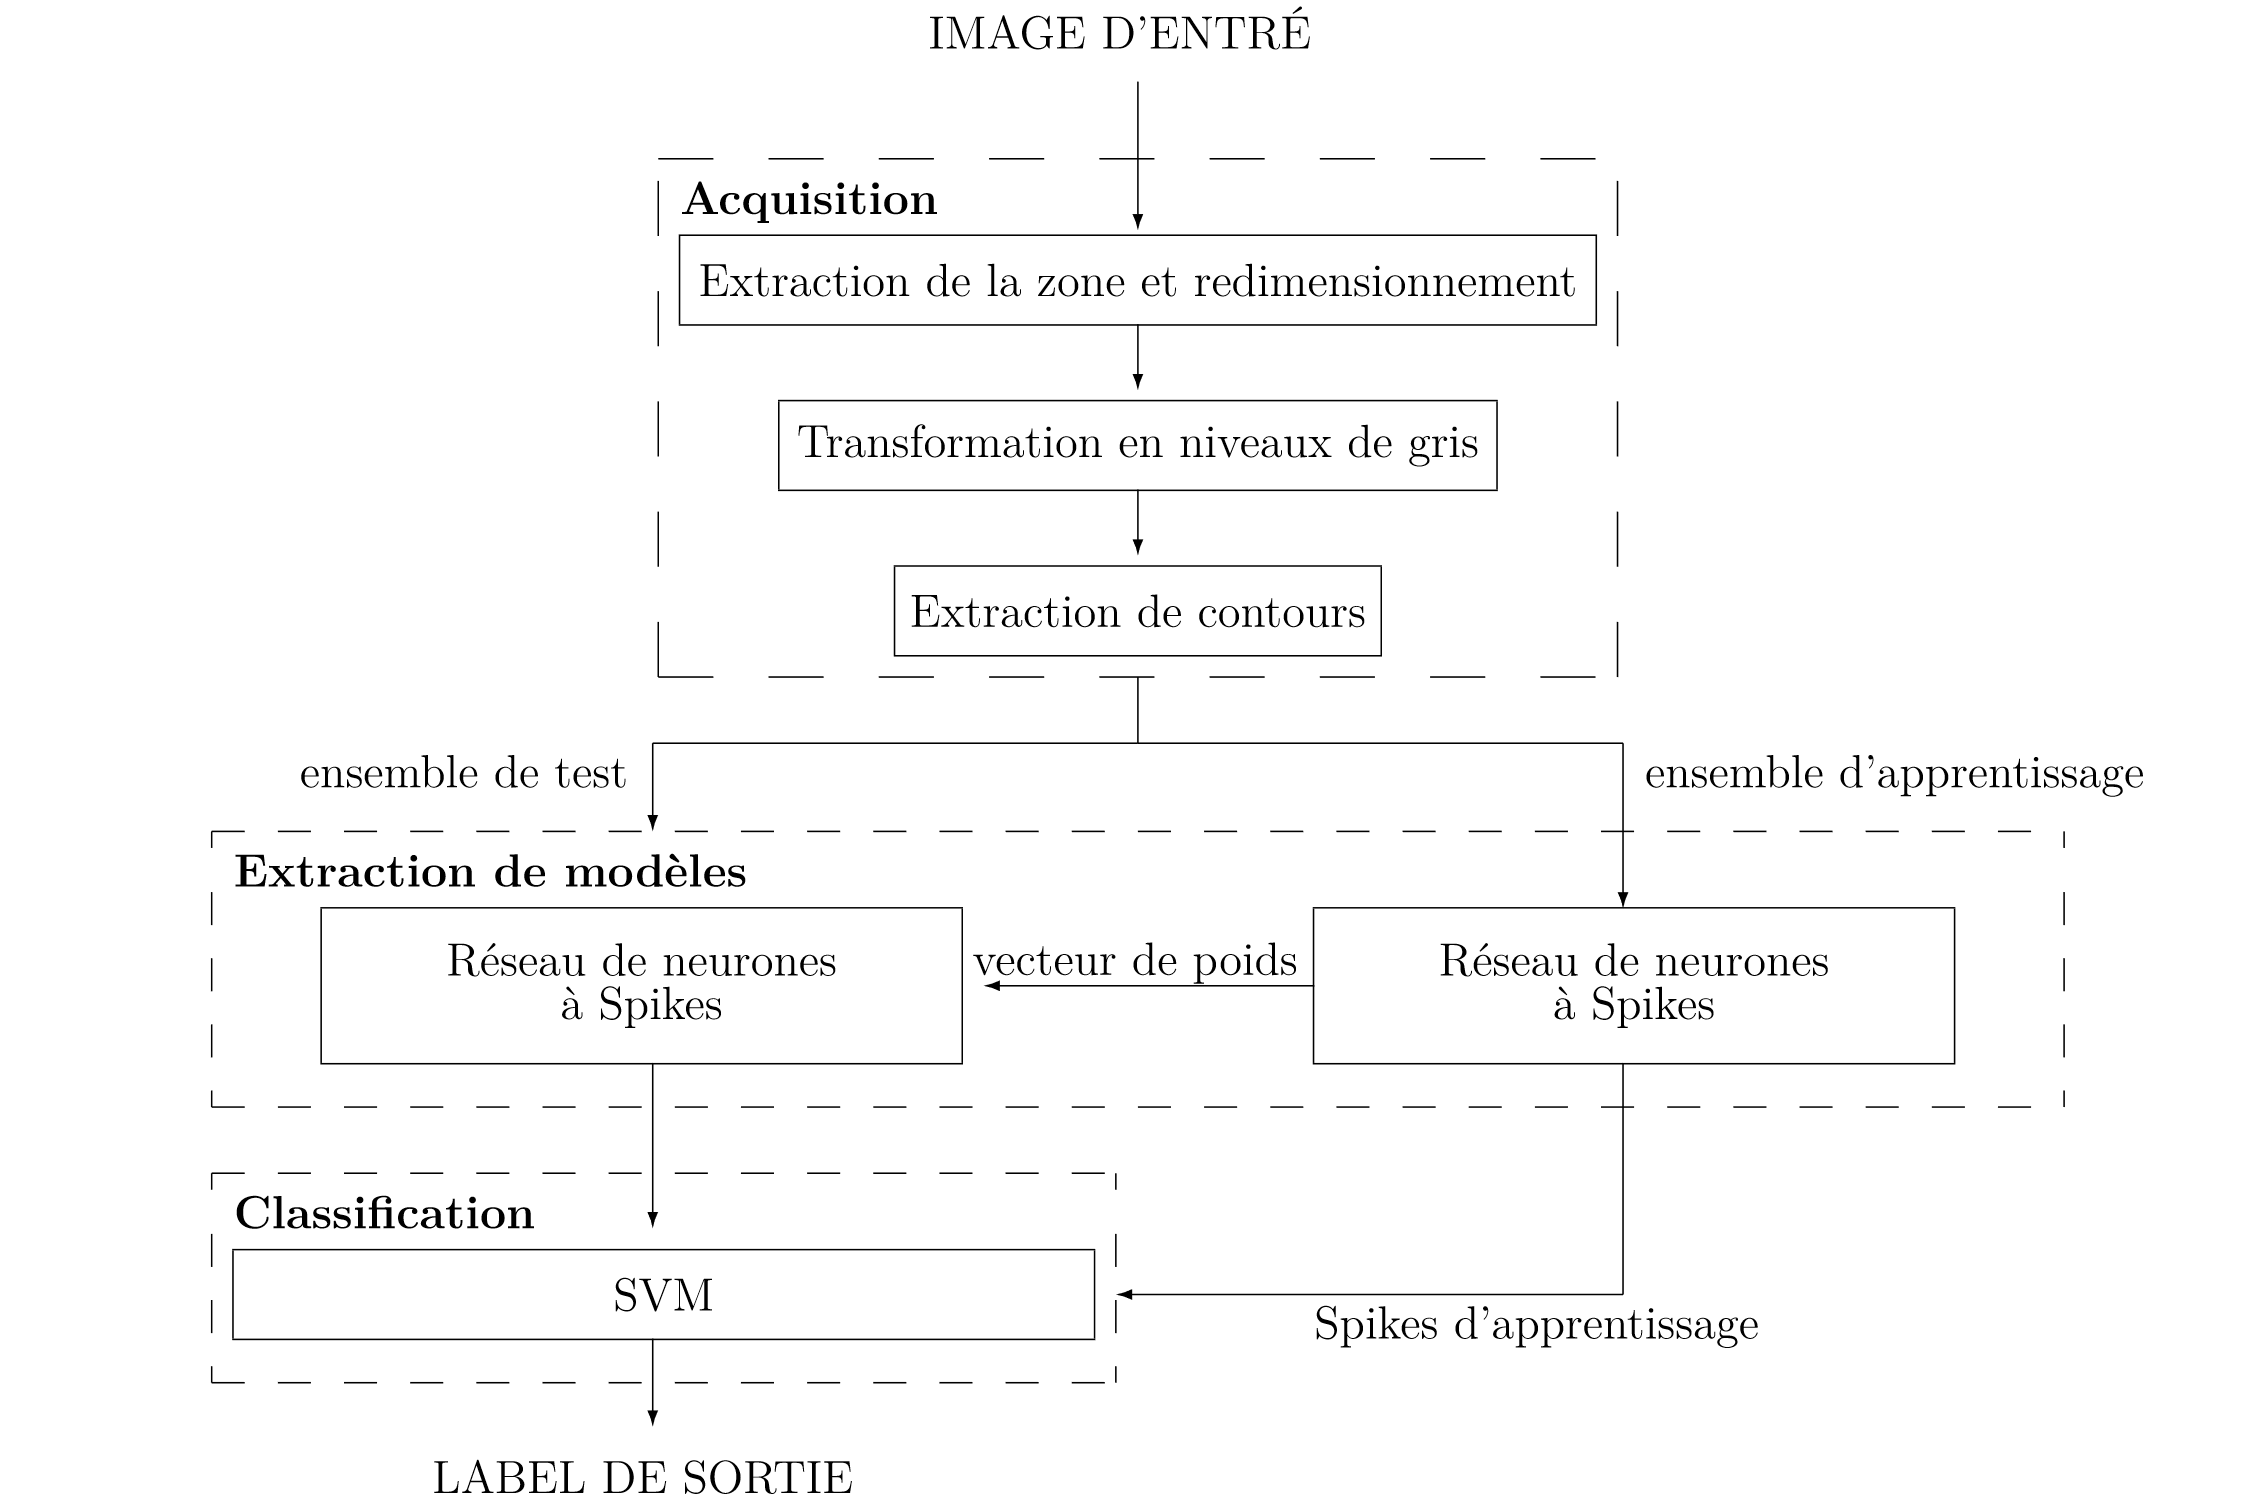
\includegraphics[scale=0.13]{image/archi.png}
  \end{figure}
\end{frame}

%------------------------------------------------

\section{Conclusion}
\begin{frame}
  \frametitle{Conclusion}
  \centering
  \begin{itemize}
  \item Un résumé
  \item Une ouverture
  \item Une expérience personnelle
  \end{itemize}
\end{frame}

%------------------------------------------------

\end{document}